\documentclass[tikz,border=2pt]{standalone}
\renewcommand{\familydefault}{\sfdefault}
\usetikzlibrary{arrows.meta,calc,positioning}
\tikzset{every picture/.style={line width=1pt, >=Stealth},
         hl/.style={fill=black, fill opacity=0.12, text opacity=1}}
\begin{document}
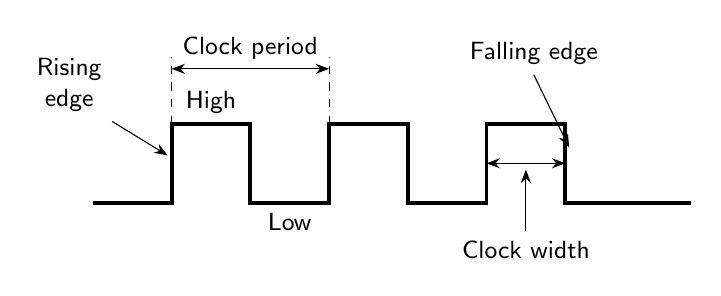
\begin{tikzpicture}[x=1cm, y=1cm, note/.style={font=\small}]
  % A square wave: high for the first half of each period, low for the second.
  \draw[line width=1.4pt] (0, 0) \foreach \t in {1, 3, 5} {-- (\t, 0) -- (\t, 1) -- (\t + 1, 1) -- (\t + 1, 0)} -- (7.6, 0);
  \node[note, above] at (1.5, 1) {High};
  \node[note, below] at (2.5, 0) {Low};
  \draw[<->, thin] (1, 1.7) -- node[note, above] {Clock period} (3, 1.7);
  \foreach \x in {1, 3} \draw[thin, dashed] (\x, 1) -- (\x, 1.85);
  \node[note, align=center] (rise) at (-0.3, 1.5) {Rising \\ edge};
  \draw[->, thin] (rise.south east) -- (0.95, 0.6);
  \node[note] (fall) at (5.6, 1.9) {Falling edge};
  \draw[->, thin] (fall.south) -- (6.05, 0.7);
  \draw[<->, thin] (5, 0.5) -- (6, 0.5);
  \node[note] (width) at (5.5, -0.6) {Clock width};
  \draw[->, thin] (width.north) -- (5.5, 0.42);
\end{tikzpicture}
\end{document}
